\chapter{When transitions are uniform POIBMDPs are fully observable}
In this section we show that decision tree induction for classification problems can be formulated as solving POIBMDPs.
Indeed, a classification problem can be formulated as an MDP where actions are class labels and states are training data.
The reward at every step is 1 if the correct label was predicted and 0 otherwise.
In this MDP, the transitions are independent of the actions: the next state is given by uniformly sampling a new training datum. 

The main result of our work is to show that when using the IBMDP framework to learn a DT for a supervised classification task, there is no need to use partially observable RL and that it is sufficient to use classical RL. We first define a new MDP and then show that a policy maximizing the expected cumulative reward of this MDP also maximizes the IBMDP reward. 

\subsection{Observation-IBMDP}
\label{sec:oibmdp}
Let us consider a base Classification MDP $\langle \mathcal{X}, \{C_1, ..., C_K\}, R, T, \gamma \rangle$ 
and an associated IBMDP $\langle S, O, A, A_{info}, R, \zeta, T_{info}, T, T_0 \rangle$. An Observation-IBMDP (OIBMDP) $\langle \Omega, A, A_{info}, R^{\prime\prime}, T^{\prime\prime}, \zeta, \gamma \rangle$ is defined as follows:

\paragraph{State space}
\vskip -0.1in
The state space is the space of possible feature bounds $\Omega \subsetneq [0,1]^{2d}$.

\paragraph{Action space} 
\vskip -0.1in
The action space is $A_{info}$, the same as in the given IBMDP.

\paragraph{Reward function}
\vskip -0.1in
Assume the current state of the MDP is $o = (L_1, ..., L_d, U_1, ..., U_d)$.
\begin{itemize}
    \item $a \in A_{info}$ : The reward for taking an IGA is still $\zeta$.
    \item $a = C_h \in \{C_1, ..., C_K\}$:  We denote $\mathcal{X}^{C_h}_{o}$ the set of all $x_i$ such that $y_i = C_h$ and $ L_k \leq x_{ik} \leq U_k$ for all $k$. Similarly, we denote $\mathcal{X}^{\bar{C_h}}_{o}$ the set of all $x_i$ such that $y_i \neq C_h$ and $ L_k \leq x_{ik} \leq U_k$ for all $k$. So $R^{\prime\prime}(o, C_h) = \frac{|\mathcal{X}^{C_h}_{o}|- |\mathcal{X}^{\bar{C_h}}_{o}|}{|\mathcal{X}^{C_h}_{o}| +|\mathcal{X}^{\bar{C_h}}_{o}|}$
\end{itemize}

\paragraph{Transition function}
Assume the current state is $o = (L_1, ..., L_d, U_1, ..., U_d)$.
\begin{itemize}
    \item $a = C_h \in \{C_1, ..., C_K\}$: $T^{\prime\prime}(o, C_h, (0,..., 0, 1, ...,1)) = 1$
    \item $a = (k, \frac{u}{p+1})\in A_{info}$: We denote $v = \frac{u}{p+1}(U_k - L_k) + L_k$. The MDP will transit to $o_{inf} = (L_1, ..., v, ..., L_d, U_1, ..., U_d)$  (resp. $o_{sup} = (L_1, ..., L_d, U_1, ..., v, ..., U_d)$) with probability $\frac{|\mathcal{X}_{o_{inf}}|}{|\mathcal{X}_{o_{inf}}| + |\mathcal{X}_{o_{sup}}|}$ (resp. $\frac{|\mathcal{X}_{o_{sup}}|}{|\mathcal{X}_{o_{inf}}| + |\mathcal{X}_{o_{sup}}|}$)
\end{itemize}

\begin{figure}
    \centering
    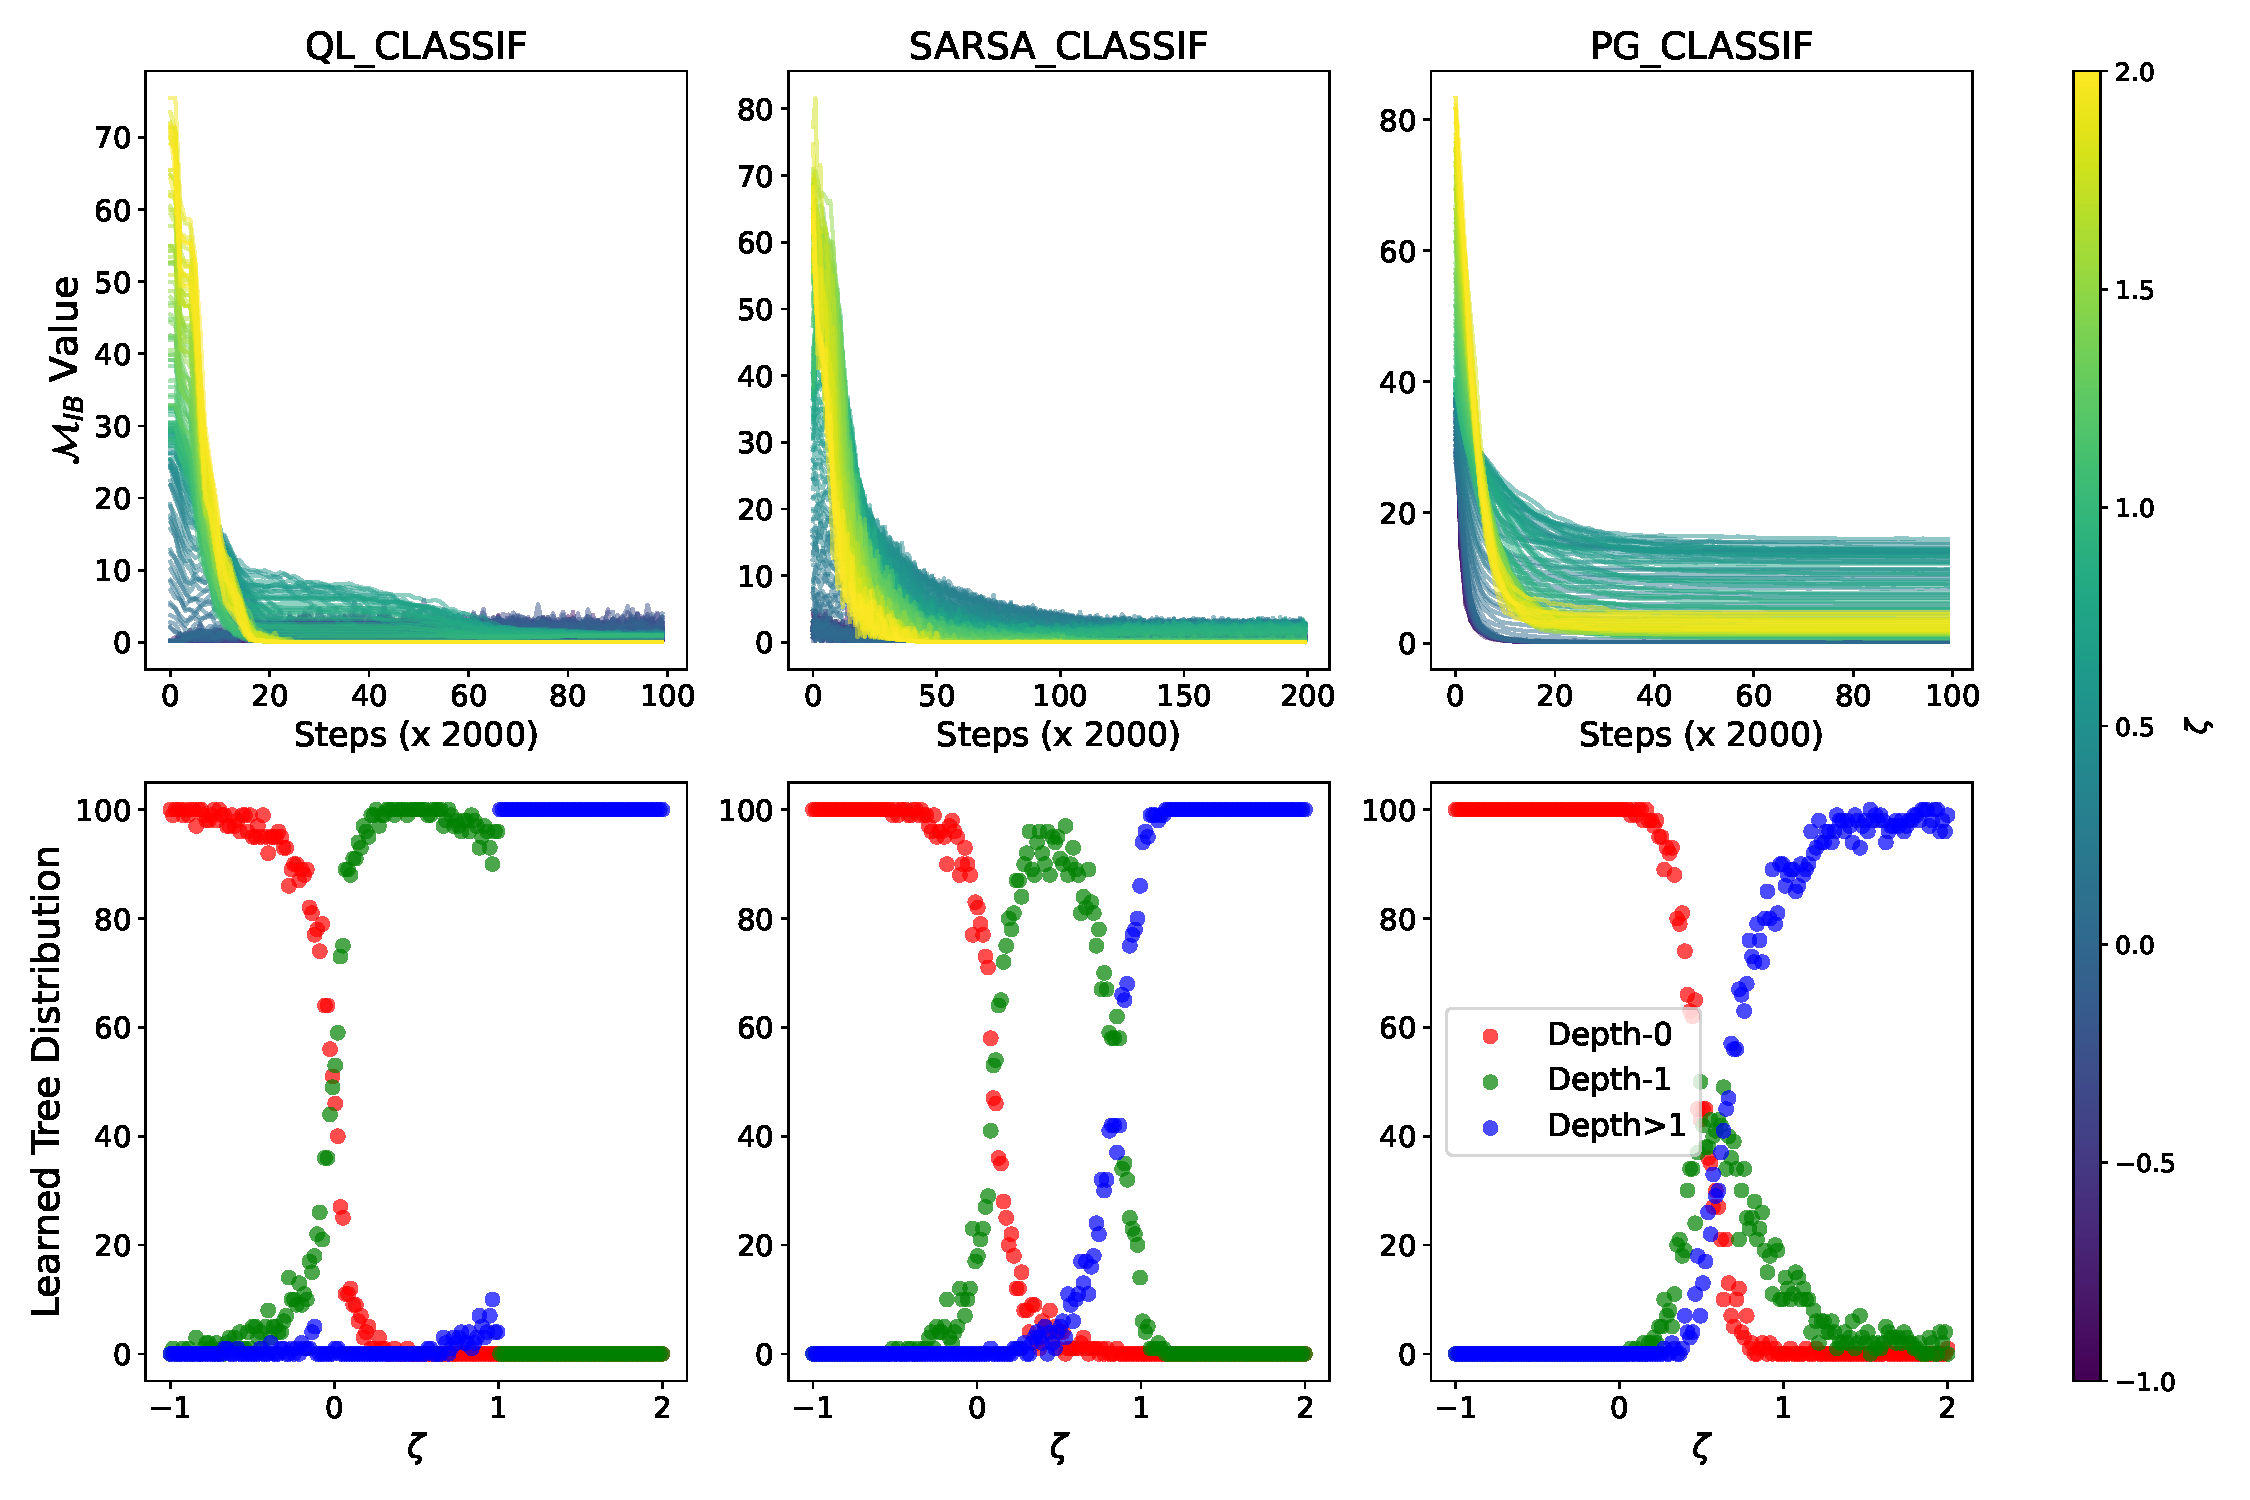
\includegraphics[width=1\textwidth]{images/images_part1/quick_plot_combined_classif.pdf}
    \caption{RL algorithms for classification OIBMDPs}\label{fig:rl-poibmdp}
\end{figure}
